\documentclass[10pt,conference,compsocconf]{IEEEtran}

%\usepackage{times}
%\usepackage{balance}
\usepackage{hyperref}

\usepackage{graphicx}	% For figure environment
\graphicspath{{./images/}}

\usepackage[numbers]{natbib}

\usepackage{caption}
\captionsetup[table]{labelfont=bf, labelsep=period}
\captionsetup[figure]{labelfont=bf, labelsep=period}

\begin{document}
\title{Road Segmentation}

\author{
  Meet Vora, Rubin Deliallisi, Rupanshu Ganvir, Vignesh Ram \\
  Group Name: Yahoo \\
  Department of Computer Science, ETH Zurich, Switzerland
}

\maketitle

\begin{abstract}
In this work, we demonstrate that road segmentation from aerial images can be effectively carried out with an end-to-end convolutional neural network. We attempt the problem from basic approaches, inspired by computer vision approaches, and then proceed to scale the models with recent deep learning approaches. We see that fully convolutional networks outperform our computer-vision approaches and help us achieve a F1 score of 0.90519 and 0.89024 on public and overall leaderboard respectively. 
\end{abstract}

\section{Introduction}


\section{Related Work}
\label{sec:related}


\section{Models and Methods} \label{sec:models-and-methods}
In this section we describe data pre-processing techniques, model architectures and the post-processing methods that we apply to our model outputs.

\subsection{Baseline} \label{subsec:baseline}
For our baseline model, we split each of our images and masks in disjoint patches of size $16 \times 16$. We then normalize each image patch by subtracting the mean and dividing by the standard deviation across our training set. To compute the patch label, we compute the mean across the mask patch and set the label to $1$ (road) if the mean is bigger than $0.25$ and $0$ (not road) otherwise.

These patches are used to train a convolutional neural network. The exact architecture is described in \autoref{tab:baseline}.

\begin{table}[h]
    \centering
    \begin{tabular}{|c|c|c|}
        \hline
        Conv(filters=$32$, kernel=$5 \times 5$) & MaxPool(kernel=$2 \times 2$) & BatchNorm \\
        \hline
        \hline
        Conv(filters=$64$, kernel=$5 \times 5$) & MaxPool(kernel=$2 \times 2$) & BatchNorm \\
        \hline
        \hline
        Dense(units=$512$, activ.=ReLU) & BatchNorm &  \\
        \hline
        \hline
        Dense(units=$1$, activ.=Sigmoid) & & \\
        \hline
    \end{tabular}
    \caption{Architecture of our baseline CNN model.}
    \label{tab:baseline}
\end{table}

\subsection{Better Baseline} \label{subsec:better-baseline}
Here we borrow from the ideas presented in \cite{Mni10}. We use a much bigger patch of size $64 \times 64$ to predict the middle $16 \times 16$ patch. This gives our model more information and hence a better prediction is expected. Similarly to \autoref{subsec:baseline}, we split each image in disjoint patches of size $64 \times 64$, using $0$ padding on the edges. Image patch normalization, mask patch extraction and label computation are identical to what we did in \autoref{subsec:baseline}.

To predict the labels, we use a convolutional neural network. The exact architecture is described in \autoref{tab:better-baseline}.

\begin{table}[h]
    \centering
    \begin{tabular}{|c|c|c|}
        \hline
        Conv(filters=$32$, kernel=$3 \times 3$) & MaxPool(kernel=$2 \times 2$) & BatchNorm \\
        \hline
        \hline
        Conv(filters=$64$, kernel=$3 \times 3$) & MaxPool(kernel=$2 \times 2$) & BatchNorm \\
        \hline
        \hline
        Conv(filters=$64$, kernel=$3 \times 3$) & MaxPool(kernel=$2 \times 2$) & BatchNorm \\
        \hline
        \hline
        Conv(filters=$128$, kernel=$3 \times 3$) & MaxPool(kernel=$2 \times 2$) &BatchNorm \\
        \hline
        \hline
        Dense(units=$512$, activ.=ReLU) & BatchNorm &  \\
        \hline
        \hline
        Dense(units=$1$, activ.=Sigmoid) & & \\
        \hline
    \end{tabular}
    \caption{Architecture of our improved baseline CNN model.}
    \label{tab:better-baseline}
\end{table}

After obtaining the results from the CNN we tried incorporating the continuous road structure in our prediction. We group our labels into $7 \times 7$ patches and use these groupings to refine the prediction of the middle label.

We use an SVM with a radial basis function kernel as our post processing model. This different from what was done in \cite{He15} where a CNN was used.

\subsection{Fully convolutional neural network (Unet)} \label{subsec:unet}
Our best performing models in this task are fully convolutional networks. First we tried Unet as introduced in \cite{Ron15}. One of the advantages of these type of networks is that they don't need enormous amounts of data to yield excellent results.

Contrary to the baseline models, we can feed the entire image to the network and backpropagate the loss from the entire mask. Nevertheless, some pre-processing is necessary. We scale all our images to the $[0,1]$ interval and normalize the data with the channel-wise mean and standard deviation of the ImageNet \cite{Imagenet} dataset. This type of normalization is necessary because we use a model pre-trained on this particular dataset. The data is further augmented with random rotations, flips, crops and scaling.

Unet is very flexible. It allows us to try different CNN architectures in its contracting and expanding paths. Among the ones we experimented with were: VGG \cite{Zis14} and ResNet \cite{He15}.

The masks generated by the network needed further processing in order to convert them into $16 \times 16$ patch predictions. We tried averaging the model output directly in each patch and applying a threshold or applying the threshold twice, once on the pixel level and once on the mask patch average level.

\subsection{Fully convolutional neural network (FCN)} \label{subsec:fcn}
The most successful model among the ones we experimented with was the FCN based on \cite{Lon14}. Its slightly older than Unet but it shares most of its characteristics.

The preprocessing part is identical to \autoref{subsec:unet}. The model we use, is also pre-trained on the ImageNet dataset. The only addition in this phase is the random noise that we add to every image before we feed it to the model. This is done to prevent over-fitting. We noticed that this model was much more prone to over-fit than Unet.

FCN is also very flexible. We could choose from several CNN architectures in its contracting and expanding paths, pre-trained on different datasets. However, we experimented only with the ResNet variants as they proved easier to train.

\section{Training and Results}
The metric that we use to evaluate our models is the F1 score.

\subsection{Baseline models} \label{subsec:training-baselines}
We trained our baseline models from scratch. After extracting the patches and corresponding labels we had $62500$ training data points. We tried data augmentation procedures such as rotations and adding noise, but these procedures did not help in this case. We use Adam with a $0.001$ learning rate and no decay as our optimizer. The batch size is fixed at $32$.

One important property of our data is class imbalance. We have roughly $3$ times more background patches than road patches. In the current literature, there are two common ways to solve this issue, modifying the training dataset or using weighted loss functions. We opted for the latter and used weighted binary cross-entropy as our loss function.

These models always achieved the best results within the first 10 epochs of training. The simpler baseline model managed to score 0.794 on the test set. The better baseline model scored 0.841 when no post-processing was applied. When SVM post-processing was applied, we achieved a slightly increased score of 0.851. A summary of these finding can be found in \autoref{tab:baseline-results}.

\begin{table}[h]
    \centering
    \begin{tabular}{|c|c|}
        \hline
        \textbf{Model} & \textbf{F1 score} \\
        \hline
        \hline
        Simple Baseline (no augmentation) & 0.794 \\
        \hline
        Simple Baseline (with augmentation) & 0.792 \\
        \hline
        Improved Baseline (no post-processing) & 0.841 \\
        \hline
        Improved Baseline (SVM post-processing) & 0.851 \\
        \hline
    \end{tabular}
    \caption{F1 score of the various baseline models.}
    \label{tab:baseline-results}
\end{table}

\subsection{Fully convolutional neural networks} \label{subsec:training-fcn}
The models used for this part are pre-trained on the ImageNet or MS-COCO datasets. We attempted to train VGG based models from scratch, but this resulted in significantly lower scores. For this type of models we have only 100 images available so data augmentation was essential. The optimizer choice was Adam with a learning rate of $0.001$ and no weight decay. The batch size is fixed at $16$ for UNet, but only $2$ for the FCN and DeepLabV3 models (because of GPU memory limitations).

As we did in \autoref{subsec:training-baselines}, we use the loss function to combat class imbalance. We experimented with weighted/unweighted binary cross entropy and the Jaccard loss. However, we found that the type of loss did not affect the prediction quality. Here we report only the results obtained by using binary cross-entropy.

We train these models for 125 epochs each. The UNet (VGG) model trained from-scratch managed to score 0.843 on the test set and 0.871 when using a pre-trained model. When using a pre-trained UNet (ResNet) model we were able to achieve an F1 score of 0.892. Our pre-trained FCN (ResNet) achieved a score of 0.904 on the test set. We achieve similar scores with DeepLabV3 (0.902) and ensemble (0.904) as well. A summary of these finding can be found in \autoref{tab:fcn-results}.

The variant of ResNet used throughout was the 101 layer one. We experiment with 34 or 50 layer networks, but found that the performance gain by using deeper networks was worth the extra training time.


\begin{table}[h]
    \centering
    \begin{tabular}{|c|c|c|c|}
        \hline
        \textbf{Model} & \textbf{Backbone} & \textbf{Pretrained} & \textbf{F1 score} \\
        \hline
        \hline
        Unet & VGG & No & 0.843 \\
        \hline
        Unet & VGG & Yes & 0.871 \\
        \hline
        Unet & ResNet & Yes & 0.892 \\
        \hline
        FCN & ResNet & Yes & 0.905 \\
        \hline
        DeepLabv3 & ResNet & Yes & 0.902 \\
        \hline
        Ensemble (FCN + DeepLabv3) & ResNet & Yes & 0.904 \\
        \hline
    \end{tabular}
    \caption{F1 score of the various fully convolutional networks.}
    \label{tab:fcn-results}
\end{table}


\section{Discussion}
\begin{figure}[h]
    \centering
    \begin{tabular}{cc}
        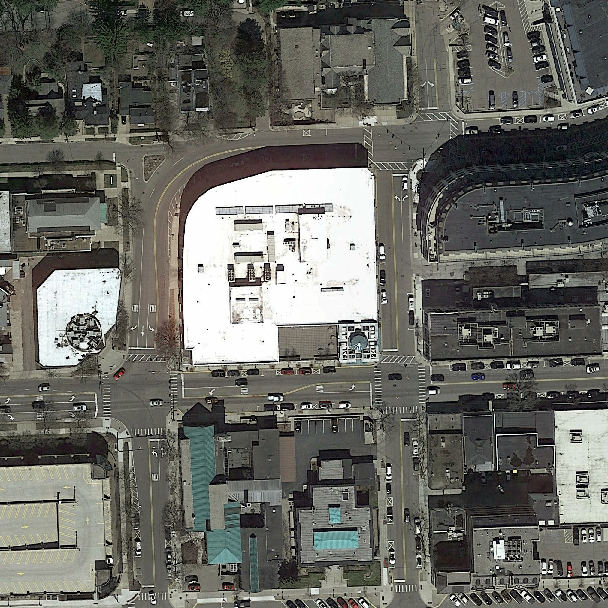
\includegraphics[width=0.4\linewidth]{original.png} & 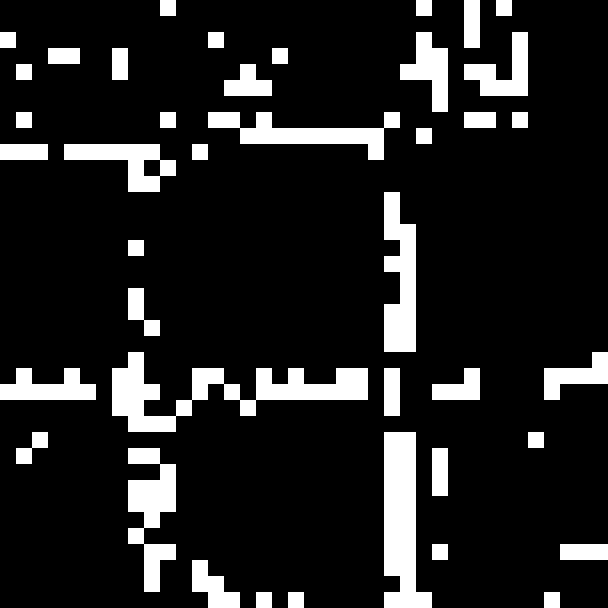
\includegraphics[width=0.4\linewidth]{baseline.png} \\
        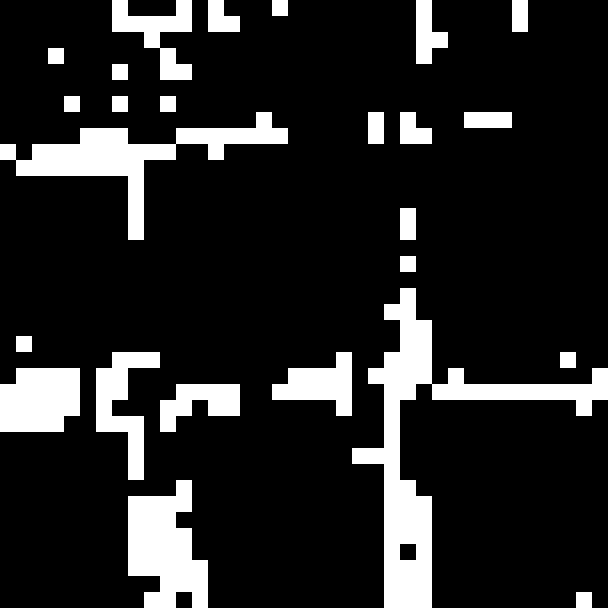
\includegraphics[width=0.4\linewidth]{baselinepp.png} & 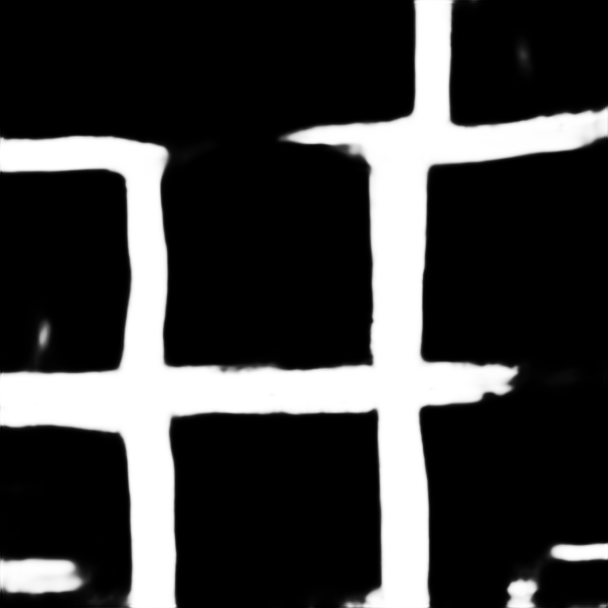
\includegraphics[width=0.4\linewidth]{fcn.png} \\
    \end{tabular}
    \caption{Top left original image. Top right baseline prediction. Bottom left better baseline prediction. Bottom right FCN prediction.}
    \label{fig:results}
\end{figure}

The baseline CNN model is by far the worst model for this task. The $16 \times 16$ patches used with this architecture contain far too little information to make an educated guess. This is true even for the trained human eye. In \autoref{fig:results} its clear that this model suffers from an abundance of false positives and false negatives.

Using $64 \times 64$ patches as we did in our second baseline model helped a tremendous amount. The larger patch size provides the model more context. Post-processing the input, whether with an SVN or a CNN helped but not significantly. We noticed that improvements of the initial predicting model impacted the performance of the post-processing model, but not vice-versa. In \autoref{fig:results} the results are slightly better than the baseline model. There is more structure to the data and less false positives. However, there are big structural gaps and a large amount of false negatives.

Fully convolutional architectures proved to be much more powerful than traditional CNN approaches. Even though we are not directly optimizing patch label prediction, better per pixel label prediction led to a better patch label prediction. As for the network type, Unet or FCN, we see very similar results at the high end and further data is needed to make a thorough comparison. The results of this model are shown in \autoref{fig:results}.

Pre-trained networks on much bigger datasets, such as ImageNet, significantly improved performance. These networks allowed us to use much deeper architectures, like the 101 layer ResNet, which would have been impossible to train with our tiny dataset.

\section{Summary}



\bibliographystyle{IEEEtranN}
\bibliography{bibliography}
\end{document}
